%%
%% This is file `sample-sigconf-authordraft.tex',
%% generated with the docstrip utility.
%%
%% The original source files were:
%%
%% samples.dtx  (with options: `all,proceedings,bibtex,authordraft')
%%
%% IMPORTANT NOTICE:
%%
%% For the copyright see the source file.
%%
%% Any modified versions of this file must be renamed
%% with new filenames distinct from sample-sigconf-authordraft.tex.
%%
%% For distribution of the original source see the terms
%% for copying and modification in the file samples.dtx.
%%
%% This generated file may be distributed as long as the
%% original source files, as listed above, are part of the
%% same distribution. (The sources need not necessarily be
%% in the same archive or directory.)
%%
%%
%% Commands for TeXCount
%TC:macro \cite [option:text,text]
%TC:macro \citep [option:text,text]
%TC:macro \citet [option:text,text]
%TC:envir table 0 1
%TC:envir table* 0 1
%TC:envir tabular [ignore] word
%TC:envir displaymath 0 word
%TC:envir math 0 word
%TC:envir comment 0 0
%%
%% The first command in your LaTeX source must be the \documentclass
%% command.
%%
%% For submission and review of your manuscript please change the
%% command to \documentclass[manuscript, screen, review]{acmart}.
%%
%% When submitting camera ready or to TAPS, please change the command
%% to \documentclass[sigconf]{acmart} or whichever template is required
%% for your publication.
%%
%%
\documentclass[sigconf,nonacm]{acmart}
%%
%% \BibTeX command to typeset BibTeX logo in the docs
\AtBeginDocument{%
  \providecommand\BibTeX{{%
    Bib\TeX}}}

%% Rights management information.  This information is sent to you
%% when you complete the rights form.  These commands have SAMPLE
%% values in them; it is your responsibility as an author to replace
%% the commands and values with those provided to you when you
%% complete the rights form.
% \setcopyright{acmlicensed}
% \copyrightyear{2018}
% \acmYear{2018}
% \acmDOI{XXXXXXX.XXXXXXX}
%% These commands are for a PROCEEDINGS abstract or paper.
% \acmConference[Conference acronym 'XX]{Make sure to enter the correct
%   conference title from your rights confirmation email}{June 03--05,
%   2018}{Woodstock, NY}
%%
%%  Uncomment \acmBooktitle if the title of the proceedings is different
%%  from ``Proceedings of ...''!
%%
%%\acmBooktitle{Woodstock '18: ACM Symposium on Neural Gaze Detection,
%%  June 03--05, 2018, Woodstock, NY}
% \acmISBN{978-1-4503-XXXX-X/2018/06}


%%
%% Submission ID.
%% Use this when submitting an article to a sponsored event. You'll
%% receive a unique submission ID from the organizers
%% of the event, and this ID should be used as the parameter to this command.
%%\acmSubmissionID{123-A56-BU3}

%%
%% For managing citations, it is recommended to use bibliography
%% files in BibTeX format.
%%
%% You can then either use BibTeX with the ACM-Reference-Format style,
%% or BibLaTeX with the acmnumeric or acmauthoryear sytles, that include
%% support for advanced citation of software artefact from the
%% biblatex-software package, also separately available on CTAN.
%%
%% Look at the sample-*-biblatex.tex files for templates showcasing
%% the biblatex styles.
%%

%%
%% The majority of ACM publications use numbered citations and
%% references.  The command \citestyle{authoryear} switches to the
%% "author year" style.
%%
%% If you are preparing content for an event
%% sponsored by ACM SIGGRAPH, you must use the "author year" style of
%% citations and references.
%% Uncommenting
%% the next command will enable that style.
%%\citestyle{acmauthoryear}

\usepackage{tabularx}

%%
%% end of the preamble, start of the body of the document source.
\begin{document}

%%
%% The "title" command has an optional parameter,
%% allowing the author to define a "short title" to be used in page headers.
\title{Gamifying the Studying Process}

%%
%% The "author" command and its associated commands are used to define
%% the authors and their affiliations.
%% Of note is the shared affiliation of the first two authors, and the
%% "authornote" and "authornotemark" commands
%% used to denote shared contribution to the research.
\author{Kierin Andrews}
\affiliation{%
  \department{School of Computing}
  \institution{University of Nebraska-Lincoln}
  \city{Lincoln}
  \state{Nebraska}
  \country{USA}
}
\email{kandrews4@huskers.unl.edu}
\author{Katelyn Breitbarth}
\affiliation{%
  \department{School of Computing}
  \institution{University of Nebraska-Lincoln}
  \city{Lincoln}
  \state{Nebraska}
  \country{USA}
}
\email{kbreitbarth2@huskers.unl.edu}
\author{Adam Furniss}
\affiliation{%
  \department{School of Computing}
  \institution{University of Nebraska-Lincoln}
  \city{Lincoln}
  \state{Nebraska}
  \country{USA}
}
\email{afurniss2@huskers.unl.edu}
\author{Elvin Nguyen}
\affiliation{%
  \department{School of Computing}
  \institution{University of Nebraska-Lincoln}
  \city{Lincoln}
  \state{Nebraska}
  \country{USA}
}
\email{enguyen17@huskers.unl.edu}
\author{Colin Salem}
\affiliation{%
  \department{School of Computing}
  \institution{University of Nebraska-Lincoln}
  \city{Lincoln}
  \state{Nebraska}
  \country{USA}
}
\email{csalem3@huskers.unl.edu}

%%
%% By default, the full list of authors will be used in the page
%% headers. Often, this list is too long, and will overlap
%% other information printed in the page headers. This command allows
%% the author to define a more concise list
%% of authors' names for this purpose.
%\renewcommand{\shortauthors}{... et al.}

%%
%% The abstract is a short summary of the work to be presented in the
%% article.
\begin{abstract}
This project presents the development of a full-stack educational application designed to enhance teaching methodologies through interactive quizzes that provide students with rewards for good performance. The system supports multiple question types, including multiple-choice single-select, multiple-choice multi-select, and true/false questions. Additionally, it implements access control mechanisms to ensure that only students enrolled in specific classes can take particular quizzes. Key features include separation of permissions between students and teachers, class enrollments, quiz creation, point tracking, rewards, achievements, and secure access controls. The application is built with a focus on scalability, usability, and adaptability to future enhancements. 

The project encompasses the design and implementation of both front-end and back-end components, including user interface development, API design, and database integration. By leveraging modern web technologies and best practices in software development - in particular, the explicit consideration of software architecture when making design decisions - this application provides an engaging and efficient platform for teachers and students alike. This report details the development process, key features, and future directions to demonstrate the system's potential as a robust educational tool. 
\end{abstract}

%%
%% The code below is generated by the tool at http://dl.acm.org/ccs.cfm.
%% Please copy and paste the code instead of the example below.
%%
\begin{CCSXML}
<ccs2012>
   <concept>
       <concept_id>10011007.10010940.10010971.10010972</concept_id>
       <concept_desc>Software and its engineering~Software architectures</concept_desc>
       <concept_significance>500</concept_significance>
       </concept>
 </ccs2012>
\end{CCSXML}

\ccsdesc[500]{Software and its engineering~Software architectures}

%%
%% Keywords. The author(s) should pick words that accurately describe
%% the work being presented. Separate the keywords with commas.
%\keywords{Do, Not, Us, This, Code, Put, the, Correct, Terms, for,
%  Your, Paper}
%% A "teaser" image appears between the author and affiliation
%% information and the body of the document, and typically spans the
%% page.
% \begin{teaserfigure}
%   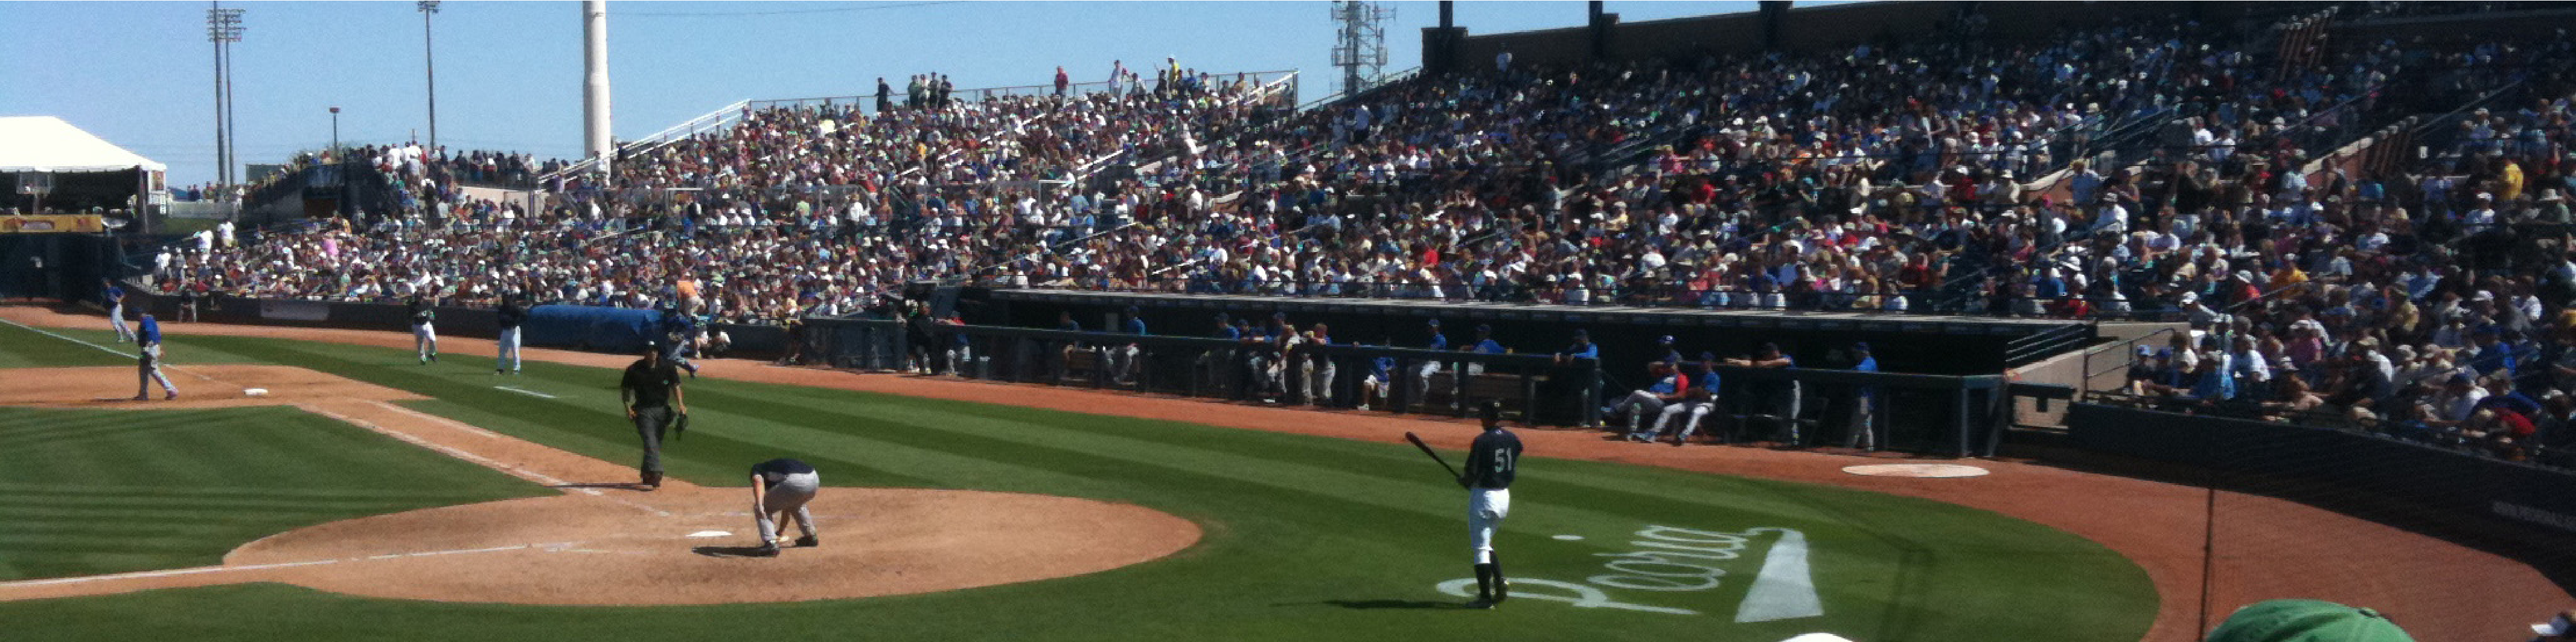
\includegraphics[width=\textwidth]{sampleteaser}
%   \caption{Seattle Mariners at Spring Training, 2010.}
%   \Description{Enjoying the baseball game from the third-base
%   seats. Ichiro Suzuki preparing to bat.}
%   \label{fig:teaser}
% \end{teaserfigure}

% \received{10 May 2025}

%%
%% This command processes the author and affiliation and title
%% information and builds the first part of the formatted document.
\maketitle

\section{Introduction}
In the educational landscape, students often struggle with inconsistent study habits, frequently resorting to cramming before exams rather than engaging in regular, spaced learning. This approach is counterproductive as it hinders deep understanding and long-term retention of information. Many existing study tools inadvertently facilitate these poor techniques by failing to provide proper motivation to students, which undermines effective learning. 

Addressing this issue is crucial because consistent study habits enable better academic performance and reinforce essential learning skills, benefiting students both academically and personally. To combat this, we have used this project as an opportunity to create a new studying platform that promotes effective learning practices, ultimately fostering sustained habits that set students up for success. 

The platform allows teachers to create quizzes for their students to take, rewarding points based on their completion and performance. These points can be redeemed for in-app rewards such as avatars, visual themes, and titles/ranks. By capping daily point earnings, the platform encourages users to return regularly and study in bursts rather than all at once, aligning with psychological findings that small, regular study sessions promote deeper learning. 

Furthermore, the architectural focus of this project ensures scalability and a smooth development process. This approach keeps our code aligned with core functionality while ensuring its capacity to grow with an increasing number of users and content. By prioritizing architecture, the project serves as a case study demonstrating the usefulness of structural design in facilitating a seamless development journey at all stages. 

This structured approach not only addresses the problem of poor study habits but also ensures that the platform is both effective and adaptable, making it accessible to a broad audience with clear and professional language.

\section{Background}
\subsection{Studying: Cramming vs. Spaced Repetition}
\label{sec:cramming-vs-spaced-repetition}
In the context of studying, cramming refers to the practice of trying to learn a large amount of information in a short period of time, often just before an exam. This method is often associated with high levels of stress and anxiety, and while it may lead to short-term retention of information, it is generally not effective for long-term learning.

For a more effective approach to studying, spaced repetition is recommended. This method involves reviewing material at increasing intervals over time, which has been shown to improve retention and understanding of the material. Spaced repetition takes advantage of the brain's natural forgetting curve, allowing learners to reinforce their memory just before they are likely to forget the information.\cite{cepeda2006distributed}

In the case of this application, the goal is to incentivize students to study in a spaced manner by allowing them to take short quizzes on the material they are learning. While they are taking the quizzes, they can earn points that can be redeemed for rewards.\cite{liu2022immediate} This approach not only encourages students to study more effectively but also provides them with immediate feedback on their understanding of the material.\cite{staddon2003operant} To further incentivize students to come back to the quizzes, points are capped at a daily limit set by their instructor. This means that students will need to return to the quizzes on multiple days in order to earn the maximum number of points possible.

\subsection{Current Solutions}
\label{sec:current-solutions}

There are several existing solutions that aim to help students study more effectively. Some of these solutions include:

\begin{itemize}
  \item Quizlet: A popular online platform that allows students to create and share flashcards, quizzes, and study games. Quizlet also offers a spaced repetition feature called "Learn" that helps students retain information over time.
  \item Kahoot!: A game-based learning platform that allows teachers to create quizzes and games for their students. Kahoot! is designed to be engaging and interactive, making it a popular choice for classroom learning.
  \item Anki: A flashcard app that uses spaced repetition to help users learn and retain information. Anki is highly customizable and allows users to create their own flashcards or download pre-made decks.
\end{itemize}

While these solutions have their strengths, they lack the "incentive" aspect that this application aims to provide. By allowing students to earn actual rewards for their studying, this application seeks to create a more engaging and motivating learning experience.\cite{smithsonian2016benefits} Additionally, the ability to set daily point caps encourages students to return to the quizzes on multiple days, further reinforcing their learning through spaced repetition.

\section{Approach}
To address the issues, our group developed a full-stack quiz application that allows students to answer questions, gain points, and earn rewards. In this section, we will discuss the system architecture, the database design, and the implementation details of our application.
\subsection{System Architecture}
Our app is built with the client-server architecture, with the front end being implemented in React.js, and the backend being implemented in Express.js. The backend communicates with the database, which is implemented using a Microsoft SQL Server (MSSQL). Authentication and session management is handled using an Express session, with the user id being stored on the server rather than on the front end in order to prevent tampering. The front end and the backend communicate via RESTful API requests, which Express handles via the Express router, communicating with the backend and returning the proper results back to the client.
\begin{figure}[H]
    \centering
    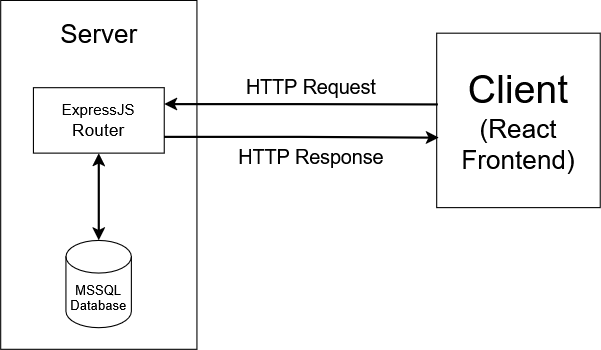
\includegraphics[width=0.7\linewidth]{PUT INDIVIDUAL SECTIONS HERE/images/clientServer(2).png}
    \caption{Client-Server Architecture of Quiz App}
    \label{client-server}
\end{figure}

\subsection{Data Modeling}
We designed our relational database schema to support users, classes, quizzes, questions, answers, and rewards. Users are able to join classes, earn points by taking quizzes associated with those classes, and then can use those points to redeem rewards.

\begin{figure}[H]
    \centering
    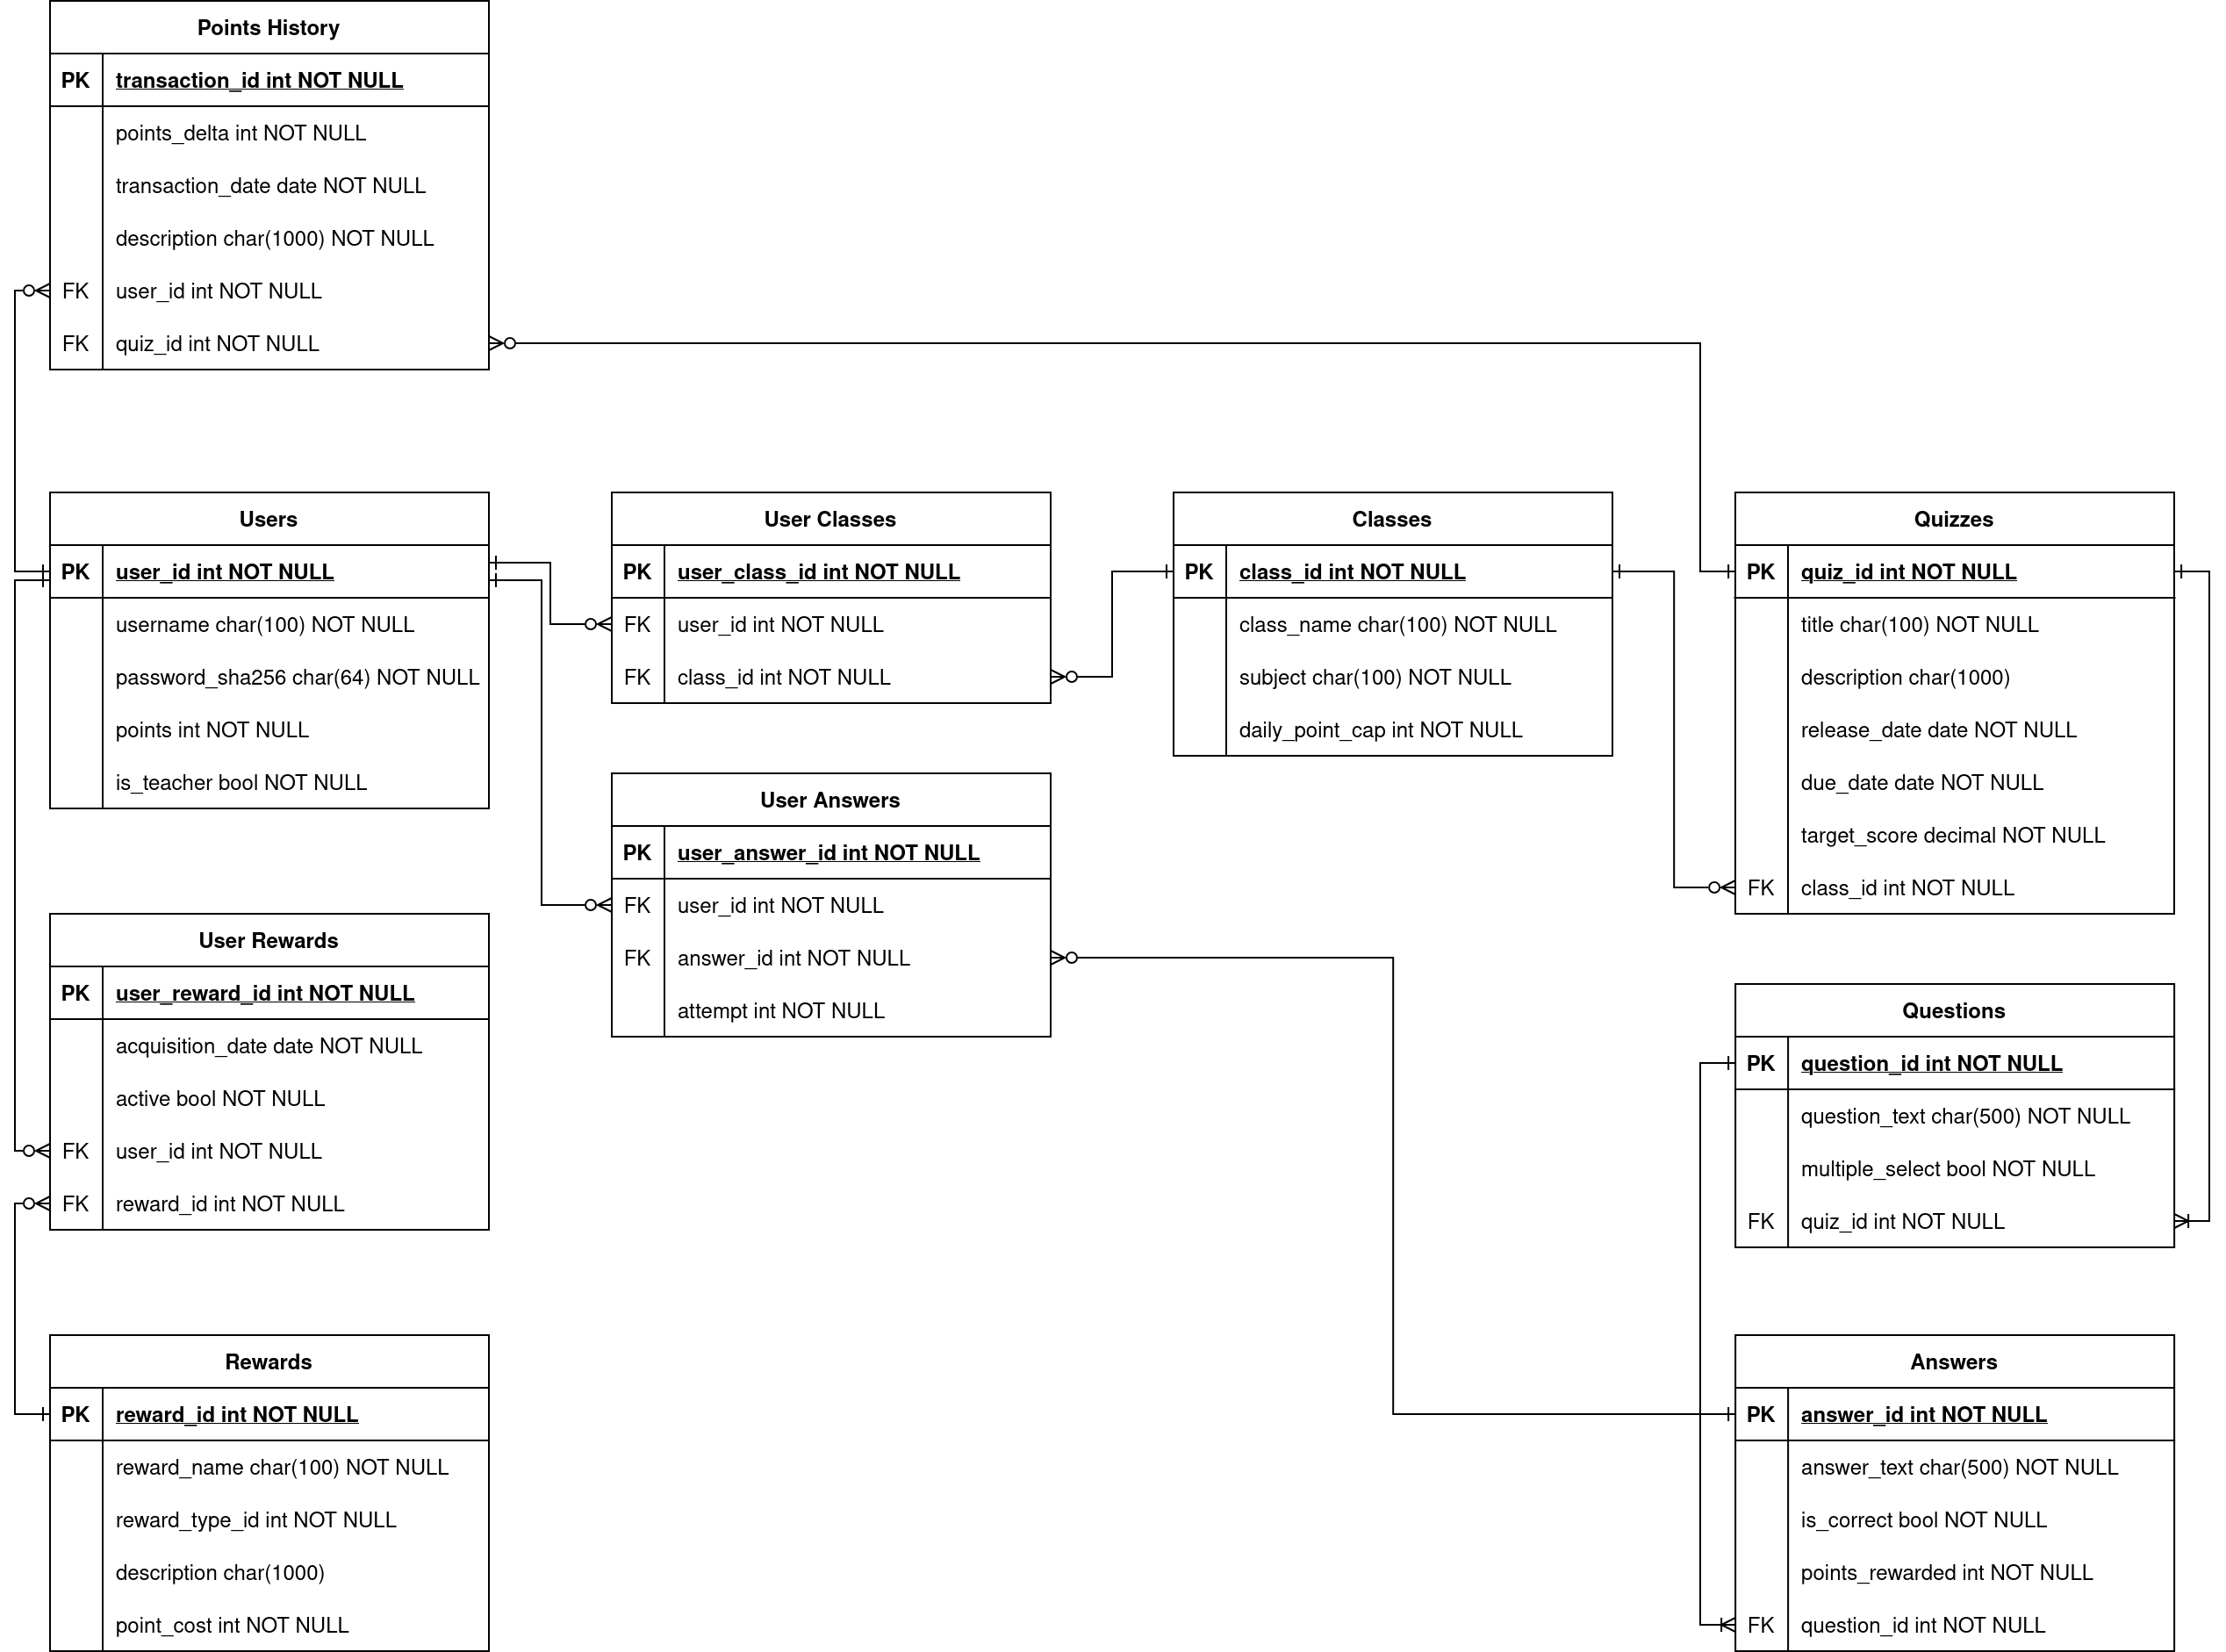
\includegraphics[width=0.7\linewidth]{PUT INDIVIDUAL SECTIONS HERE/images/466_ER_Diagram.drawio.png}
    \caption{Entity-Relationship Diagram for Database Schema}
    \label{ER-diagram}
\end{figure}

\subsection{Component Structure}
Our front end is built using React, which allows us to break up our app into modular components that each handle different functionality, making the app easier to maintain.
\begin{figure}[H]
    \centering
    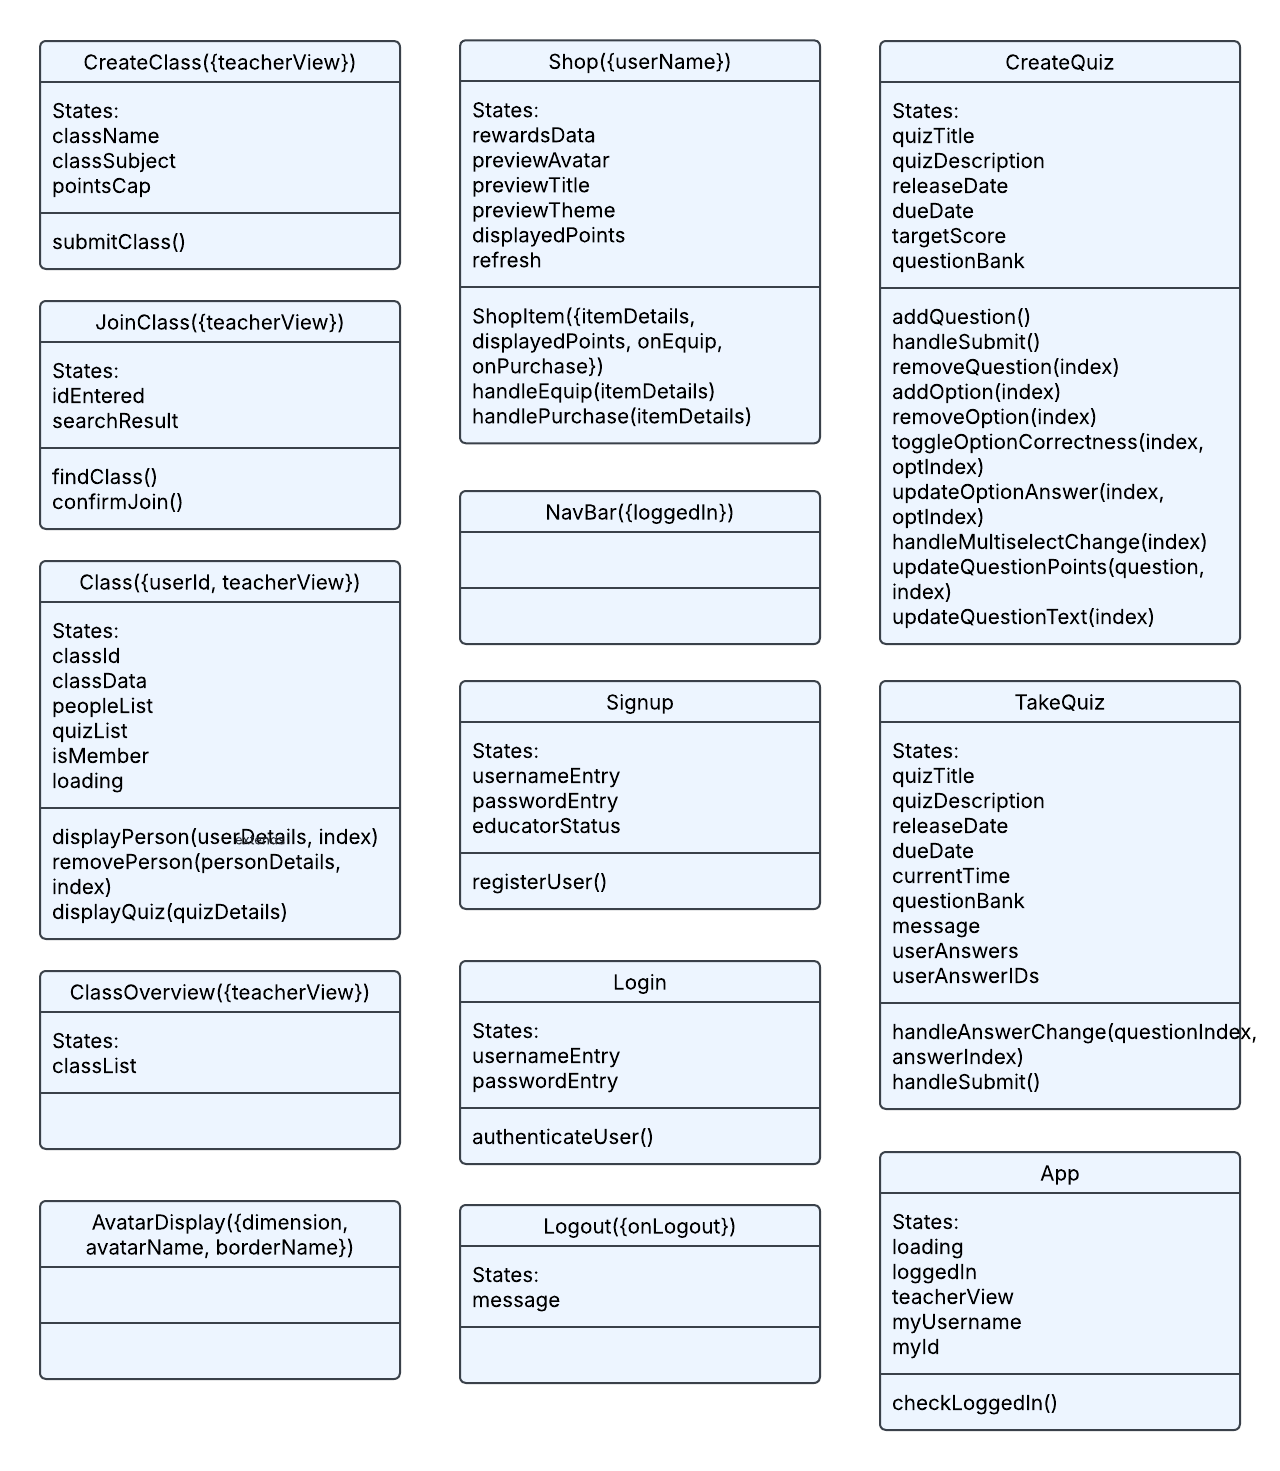
\includegraphics[width=0.7\linewidth]{PUT INDIVIDUAL SECTIONS HERE/images/UML_class.png}
    \caption{UML diagram that displays React components, states, and methods}
    \label{fig:enter-label}
\end{figure}
This diagram shows a high-level snapshot of some of the key components, including:
\begin{itemize}
    \item App - Manages global state, including login and authentication.
    \item CreateQuiz - Provides question/answer editing functionality.
    \item TakeQuiz - Renders quiz content, tracks answers, and submits completed attempts to backend.
    \item Shop - Handles reward purchasing and activation.
\end{itemize}
Business logic is handled inside each component, and most user actions result in fetch() calls to endpoints defined by the Express.js router.

\subsection{Application Walkthrough}
There are two main users that use the app, their workflows are shown below.
\subsubsection{Students}
\begin{enumerate}
    \item Students enter a class code in the JoinClass component.
    \begin{figure}[h]
        \centering
        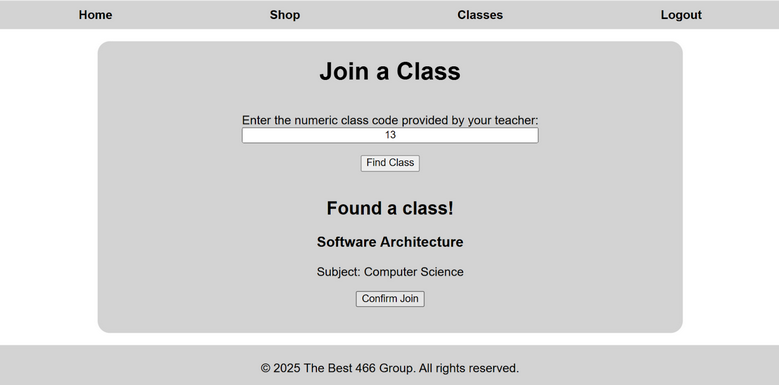
\includegraphics[width=0.7\linewidth]{PUT INDIVIDUAL SECTIONS HERE/images/joinClass.png}
        \caption{Join Class component}
        \label{join-class}
    \end{figure}
        \item Students can take quizzes assigned to them by their teachers, earning points with every correct answer.
    \begin{figure}[H]
        \centering
        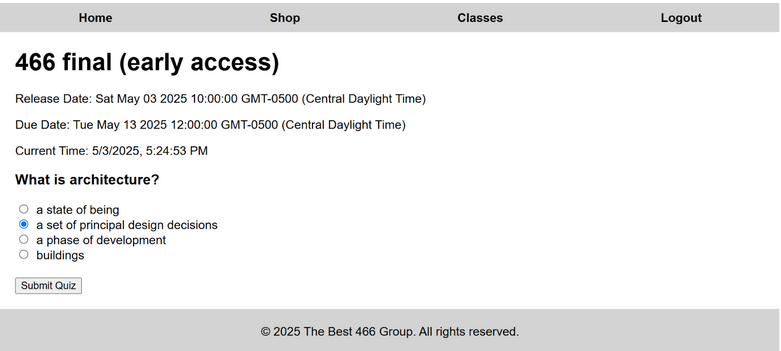
\includegraphics[width=0.7\linewidth]{PUT INDIVIDUAL SECTIONS HERE/images/TakeQuiz.png}
        \caption{Take Quiz component}
        \label{take-quiz}
    \end{figure}
        \item Students can then spend their accumulated points in the shop, earning customization features such as avatars.
\begin{figure}[H]
    \centering
    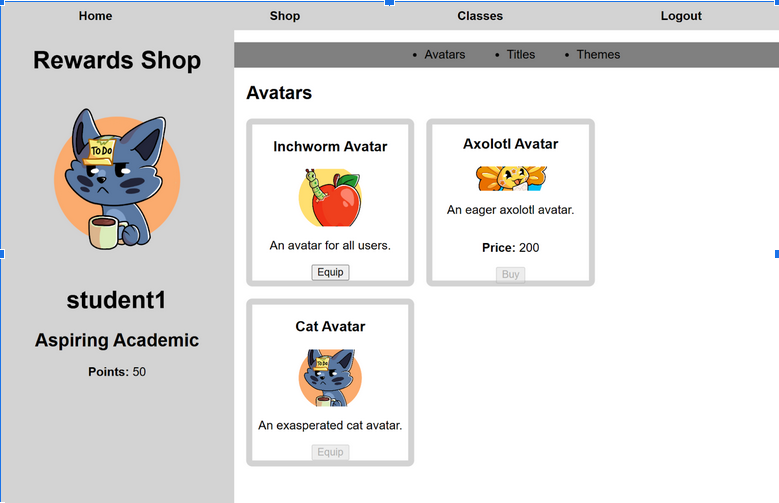
\includegraphics[width=0.7\linewidth]{PUT INDIVIDUAL SECTIONS HERE/images/Shop.png}
    \caption{Shop component}
    \label{Shop}
\end{figure}
\end{enumerate}
\subsubsection{Teachers}
\begin{enumerate}
    \item Teachers use the CreateClass component to define class name, subject, and daily point caps.
    \begin{figure}[h]
        \centering
        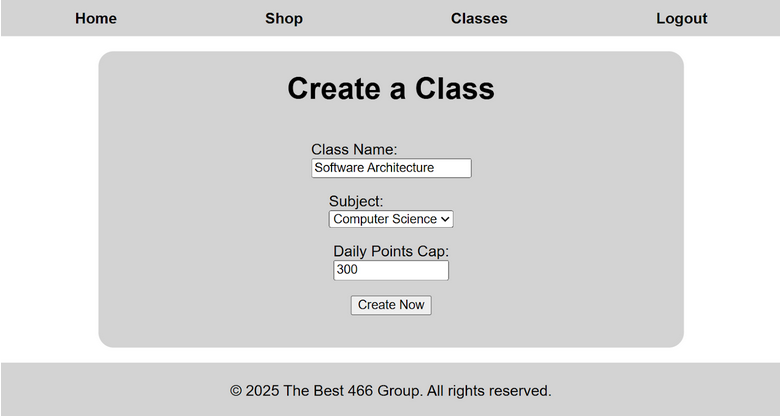
\includegraphics[width=0.7\linewidth]{PUT INDIVIDUAL SECTIONS HERE/images/createClass.png}
        \caption{Create Class component}
        \label{fig:enter-label}
    \end{figure}
        \item Teachers can view their students in with the ClassOverview component.
    \begin{figure}[H]
        \centering
        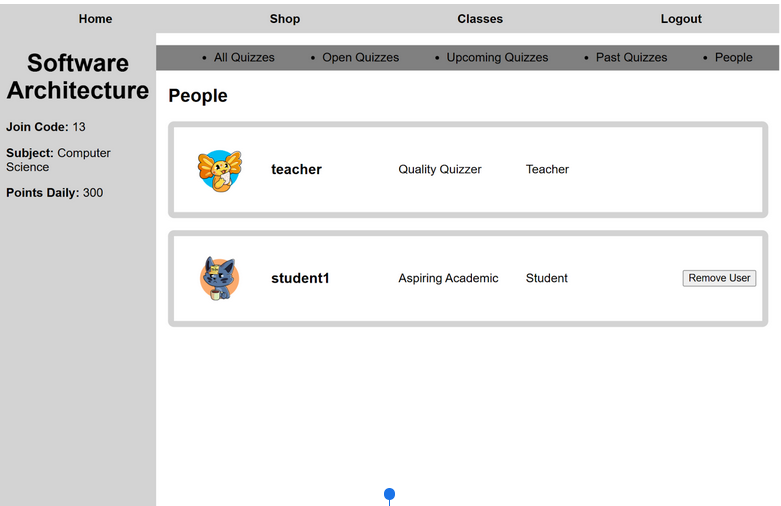
\includegraphics[width=0.7\linewidth]{PUT INDIVIDUAL SECTIONS HERE/images/classOverview.png}
        \caption{Class Overview component}
        \label{class-overview}
    \end{figure}
        \item Teachers can define quizzes with multiple questions with the CreateQuiz component. These questions support both single correct answer and multiple correct answers.
    \begin{figure}[H]
        \centering
        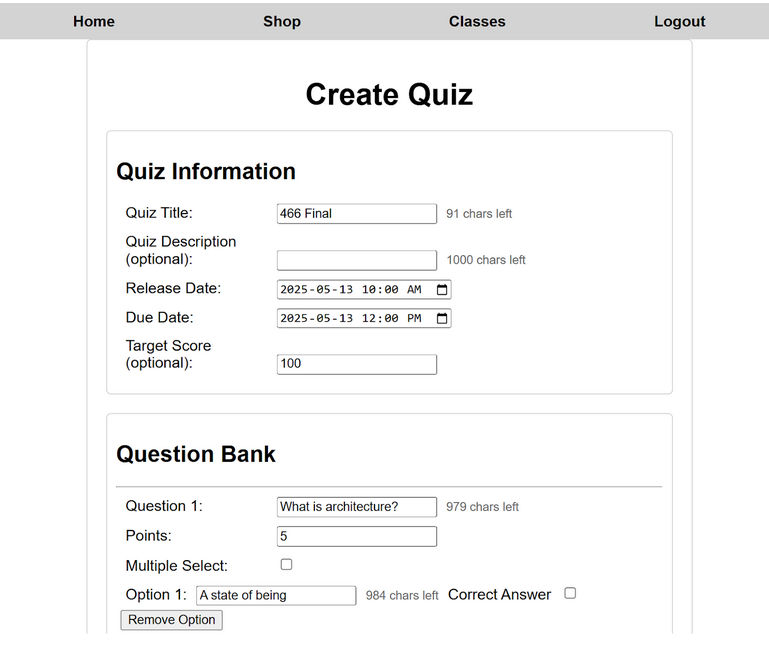
\includegraphics[width=0.7\linewidth]{PUT INDIVIDUAL SECTIONS HERE/images/createQuiz.png}
        \caption{Create Quiz component}
        \label{create-quiz}
    \end{figure}
        
\end{enumerate}
\subsection{Merit}
This tool successfully solves a number of problems mentioned in our background section. By allowing teachers the ability to create custom quizzes, teachers can successfully emphasize certain points in the curriculum, improving learning while simultaneously making life easier for teachers. For students, our app successfully supports the gamification of studying by allowing students to earn rewards for studying, turning it into a fun task rather than a chore. Our app also supports studying over time rather than cramming all at once with the introduction of a daily point cap. By introducing the cap, it encourages students to complete the quizzes on multiple days, rather than on a single day, in order to maximize their total points. Overall, our app reduces overhead for teachers, enhances student engagement, and supports classroom management.




\section{Outline of Project Plan}
The development of the software was split across four major phases:

\subsection{Requirements (3/24/25 - 3/31/35)}

During this phase, we built our initial prescriptive architecture through use of the twin peaks model. Initial requirements were collected, then used to inform our initial decision of a client-server style, then revisited under this architecture to iteratively build a cohesive, architecture-centered plan.

This section's major responsibilities included:
\begin{itemize}
    \item \textbf{Functional Requirement Identification}
    \item \textbf{Nonfunctional Requirement Identification}
    \item \textbf{Architectural Style Identification}: Evolving alongside the lists of requirements, built an initial prescriptive architecture based on the client-server style.
\end{itemize}

Deliverables for this section included a list of requirements of each type, as well as the choice of architectural style to be elaborated on in the next stage. For resources, lecture slides detailing the major architectural styles were used to find a favorable match for our requirements.

\subsection{Design (3/31/25 - 4/7/5)}

With a strong sense of our app's requirements and a favorable architecture to build them under, this phase centered on further refinement of these concepts by choosing a particular tech stack for the implementation, as well as making proper diagrams to capture the architectural decisions. The architectural decisions made in the previous phase remained at the forefront of this stage and were further refined through the creation of these explicit diagrams.

This section's major responsibilities included:
\begin{itemize}
    \item \textbf{Tech Stack Identification}: It was decided a React front-end would provide a smooth experience to users for the purposes of data entry. With this, an Express.js backend to handle the API and business logic was a natural choice. MSSQL was chosen for the server based on the team's personal familiarity.
    \item \textbf{Creation of Architecture Diagrams}: An ER diagram for the server, a UML diagram of the front-end React components, and a client-server diagram portraying the whole system were produced.
\end{itemize}

\subsection{Implementation (4/7/25 - 4/21/25)}

Here, the prescriptive architecture was put into place, with the hopes of the detail at previous phases mitigating any architectural drift that occurred. To that end, the team monitored for architectural degradation or any incompatibilities with system demands that were found as individual requirements were translated to code.

This section's major responsibilities included:
\begin{itemize}
    \item \textbf{Implementing the GUI}: This included the React components, as well as setting them up to make their API calls.
    \item \textbf{Implementing the backend}: This included the structure for the MSSQL server itself, as well as the Express.js routes to interact with it.
\end{itemize}

By the end of this phase, the app's source code was produced as a deliverable, along with a SQL script for easy server setup.

\subsection{Analysis and Testing (4/21/25 - 5/5/25)}

During this stage, the merits of our architecture-centered development were put to the test. The separation of concerns produced by following a layered architecture such as client-server were expected to greatly simplify the testing process when it came to unit tests. If we adhered to the architecture as expected, the architecture analysis conducted at this stage should reflect that.

This section's major responsibilities included:
\begin{itemize}
    \item \textbf{Implementing Unit Tests}: Unit tests on the React components ensured that our client was processing responses from the server as expected, allowing us to verify the core separateness of the layers despite their interactions.
    \item \textbf{Conducting Architecture Analysis}: Producing a writeup on the major aspects, advantages, and limitations of the architecture as it was realized.
\end{itemize}

Though these four phases used up the allotted time for initial project completion, future maintenance and evolution is expected to make full use of the architectural foundation laid by these previous phases.

\section{Evaluation}
\subsection{Architectural Overview}
The system is built on a client–server architecture, separating concerns between a \textbf{React frontend} and an \textbf{Express backend}. This modular design ensures that each component can operate, scale, and be maintained independently. The backend manages business logic and database interactions, while the frontend is responsible for presenting information and capturing user interaction. Communication between the two layers occurs exclusively via RESTful API calls, maintaining a strict separation of concerns and minimizing coupling.

\subsection{Evaluation of Key Architectural Aspects}

\textbf{Logical Separation:} The frontend and backend are completely decoupled; the frontend has no direct access to backend logic or databases.

\textbf{Communication (API):} All interactions occur via RESTful APIs, preserving a stateless design and enabling consistent decoupling.

\textbf{Security:} Authentication and authorization are handled server-side. The frontend never handles sensitive logic or has direct access to user data.

\textbf{Responsibility Split:} The client manages rendering and local UI state; the server handles data validation, persistence, and all core processing.

\subsection{Strengths}
\begin{itemize}
    \item \textbf{Scalability}: The backend can be scaled independently (e.g., through load balancing), while the frontend is lightweight and can be served statically.
    \item \textbf{Maintainability}: Clear separation of concerns allows UI changes without backend modifications and vice versa, improving long-term maintainability.
    \item \textbf{Flexibility}: The system architecture supports multiple types of clients using the same backend API.
    \item \textbf{Security}: By centralizing sensitive operations on the server, the system reduces exposure to potential vulnerabilities.
\end{itemize}

\subsection{Limitations}
\begin{itemize}
    \item \textbf{Database Integration}: Local databases are currently in use, limiting centralization and real-time synchronization between users.
    \item \textbf{Feature Scope}: Some intended features remain unimplemented due to time constraints; future iterations could further enhance system capability.
    \item \textbf{User Interface}: Functionality was prioritized over visual design, resulting in a utilitarian UI that could benefit from aesthetic improvements.
\end{itemize}

\subsection{Alignment with Project Goals}

\begin{table}[H]
\centering
\noindent\begin{tabularx}{\linewidth}{|l|X|}
\hline
\textbf{Goal} & \textbf{Implementation} \\
\hline
Sustainable Study Habits & The server enforces daily point caps to promote consistent, healthy engagement patterns. \\
\hline
Gamification and Rewards & The client displays avatars and themes based on reward data retrieved from the backend. \\
\hline
Scalability & The architecture supports increasing user loads without compromising client performance. \\
\hline
Educational Feedback & The server aggregates and processes user performance data; the client renders this feedback to users. \\
\hline
\end{tabularx}
\caption{Project Goals and Architectural Alignment}
\end{table}

\subsection{Architectural Overview}
The system is built on a client–server architecture, separating concerns between a \textbf{React frontend} and an \textbf{Express backend}. This modular design ensures that each component can operate, scale, and be maintained independently. The backend manages business logic and database interactions, while the frontend is responsible for presenting information and capturing user interaction. Communication between the two layers occurs exclusively via RESTful API calls, maintaining a strict separation of concerns and minimizing coupling.

\subsection{Evaluation of Key Architectural Aspects}

\textbf{Logical Separation:} The frontend and backend are completely decoupled; the frontend has no direct access to backend logic or databases.

\textbf{Communication (API):} All interactions occur via RESTful APIs, preserving a stateless design and enabling consistent decoupling.

\textbf{Security:} Authentication and authorization are handled server-side. The frontend never handles sensitive logic or has direct access to user data.

\textbf{Responsibility Split:} The client manages rendering and local UI state; the server handles data validation, persistence, and all core processing.

\subsection{Strengths}
\begin{itemize}
    \item \textbf{Scalability}: The backend can be scaled independently (e.g., through load balancing), while the frontend is lightweight and can be served statically.
    \item \textbf{Maintainability}: Clear separation of concerns allows UI changes without backend modifications and vice versa, improving long-term maintainability.
    \item \textbf{Flexibility}: The system architecture supports multiple types of clients using the same backend API.
    \item \textbf{Security}: By centralizing sensitive operations on the server, the system reduces exposure to potential vulnerabilities.
\end{itemize}

\subsection{Limitations}
\begin{itemize}
    \item \textbf{Database Integration}: Local databases are currently in use, limiting centralization and real-time synchronization between users.
    \item \textbf{Feature Scope}: Some intended features remain unimplemented due to time constraints; future iterations could further enhance system capability.
    \item \textbf{User Interface}: Functionality was prioritized over visual design, resulting in a utilitarian UI that could benefit from aesthetic improvements.
\end{itemize}

\subsection{Alignment with Project Goals}

\begin{table}[H]
\centering
\noindent\begin{tabularx}{\linewidth}{|l|X|}
\hline
\textbf{Goal} & \textbf{Implementation} \\
\hline
Sustainable Study Habits & The server enforces daily point caps to promote consistent, healthy engagement patterns. \\
\hline
Gamification and Rewards & The client displays avatars and themes based on reward data retrieved from the backend. \\
\hline
Scalability & The architecture supports increasing user loads without compromising client performance. \\
\hline
Educational Feedback & The server aggregates and processes user performance data; the client renders this feedback to users. \\
\hline
\end{tabularx}
\caption{Project Goals and Architectural Alignment}
\end{table}


\section{Conclusions and Future Work}
The app successfully promotes evidence-backed studying methods, such as spaced repetition, through the implementation of daily points caps. Each class has an individual cap set by the teacher at creation, allowing independence between classes and preventing students from neglecting certain classes if they've already exhausted their daily incentives. Reinforcement by earning points builds daily studying habits. Teachers can take an active role in the preparation of their students by providing tailored quizzes for their classes that target specific information deemed crucial for understanding, as well as set target scores for the created quizzes.

The primary goal that could not be completed during course time is providing analytical tools for teachers to see the performance of their students on quizzes and individual questions. These statistics may indicate widespread successes or misunderstandings that help adjust teaching methods. Records of user answers for a quiz, including on individual attempts, are already stored in the database upon quiz submission, so this would be relatively simple to implement as part of the teacher view. Pairing with this, new functionality to revise quizzes after creating them would be useful.

Beyond this, the current system is limited in that it relies on local MSSQL databases to store data. Having a single shared database would be essential if this app were released to a real user setting. Additionally, due to time constraints, image assets for the rewards are currently kept on the client side rather than pulled from the server, meaning new rewards require updates to both the server and the client’s static files. Server-side BLOB storage of these assets would be ideal to remove this dependency. As part of these server upgrades, additional input validation on client-side form fields would be required to better protect data, such as against injection attacks.

Potential expansions to functionality include enabling classes to have multiple teachers, perhaps through explicit invitation from an existing teacher rather than use of a join code, to prevent undue changes to the preexisting system architecture. Lastly, allowing teachers to reuse quizzes from other classes or adding public quizzes for all students to access would be a useful tool that matches services provided by similar studying platforms.

Finally, improving the user interface and user experience would elevate the app significantly. Functionality was prioritized over aesthetics, so the current product is very simple in appearance, at the cost of its long-term appeal. Styling the pages and providing additional visual feedback for things like button clicks would add interest and help keep users engaged. Extending the role of the rewards, such as allowing themes to influence the visual design of pages, would add to the cohesion of the app and increase the appeal of the rewards.

Overall, though there are a multitude of ways the app could continue to be developed and improved into a more complete product, the core functionality has been finished in an adaptable and architecturally sound state. Thanks to the early identification of a favorable architecture for the system in the form of the client-server style, and subsequent reframing of our requirements in this context, direction for the app was well-defined from the early stages. Subsequent stages saw us consulting and revisiting this architecture as the features were developed, allowing smooth negotiation of which layers would handle the minutiae of the implementation. Future work is expected to work smoothly within the existing system thanks to this foundation, attesting to the crucial role architecture plays in the long-term maintenance and evolution of a software system.



%%
%% The next two lines define the bibliography style to be used, and
%% the bibliography file.
\bibliographystyle{ACM-Reference-Format}
\bibliography{reportBiblio}


%%
%% If your work has an appendix, this is the place to put it.
\appendix

\section{Division of Work}


\end{document}
\endinput
%%
%% End of file `sample-sigconf.tex'.
